\documentclass[draftclsnofoot,10pt,onecolumn]{IEEEtran} %!PN

\usepackage[margin=0.5cm]{caption}
\usepackage{lipsum}

\usepackage{longtable}
\usepackage{graphicx}   
\usepackage[export]{adjustbox} 
\usepackage{epstopdf}

\usepackage{pdfpages}

\usepackage{caption}

\usepackage{amssymb}                                         
\usepackage{amsmath}                                         
\usepackage{amsthm}                                          

\usepackage{alltt}                                           
\usepackage{float}
\usepackage{color}

\usepackage{hyperref}
\usepackage{url}

\usepackage{array}

\usepackage{balance}
\usepackage[TABBOTCAP, tight]{subfigure}
\usepackage{enumitem}

\newcommand{\ignore}[2]{\hspace{0in}#2} %Used for inline comments
\newcommand{\tab}{\hspace*{2em}} %For tabbing

\usepackage{pstricks, pst-node}

\usepackage{geometry}
%\usepackage{graphicx}
\geometry{textheight=10in, textwidth=7.5in, margin=0.75in}

\usepackage{listings}

\definecolor{mygreen}{rgb}{0,0.6,0}
\definecolor{mygray}{rgb}{0.5,0.5,0.5}
\definecolor{mymauve}{rgb}{0.58,0,0.82}
\linespread{1}

\lstset{ %
  basicstyle=\ttfamily,            % the size of the fonts that are used for the code
  breakatwhitespace=false,         % sets if automatic breaks should only happen at whitespace
  breaklines=true,                 % sets automatic line breaking
  captionpos=b,                    % sets the caption-position to bottom
  commentstyle=\color{mygreen},    % comment style
  escapeinside={\%*}{*)},          % if you want to add LaTeX within your code
  extendedchars=true,              % lets you use non-ASCII characters; for 8-bits encodings only, does not work with UTF-8
  keepspaces=true,                 % keeps spaces in text, useful for keeping indentation of code (possibly needs columns=flexible)
  keywordstyle=\color{blue},       % keyword style
  %numbers=left,                    % where to put the line-numbers; possible values are (none, left, right)
  %numbersep=10pt,                  % how far the line-numbers are from the code
  %numberstyle=\tiny\color{mygray}, % the style that is used for the line-numbers
  rulecolor=\color{black},         % if not set, the frame-color may be changed on line-breaks within not-black text (e.g. comments (green here))
  showspaces=false,                % show spaces everywhere adding particular underscores; it overrides 'showstringspaces'
  showstringspaces=false,          % underline spaces within strings only
  showtabs=false,                  % show tabs within strings adding particular underscores
  stepnumber=1,                    % the step between two line-numbers. If it's 1, each line will be numbered
  stringstyle=\color{mymauve},     % string literal style
  tabsize=8,                       % sets default tabsize to 8 spaces
  %title=\lstname                  % show the filename of files included with \lstinputlisting; also try caption instead of title
}

\lstdefinelanguage{JavaScript}{
  morekeywords={var, function},
  morecomment=[s]{/*}{*/},%
  morecomment=[l]//,%
  morestring=[b]",%
  morestring=[b]'%
}

\usepackage{hyperref}

\def\BibTeX{{\rm B\kern-.05em{\sc i\kern-.025em b}\kern-.08em
    T\kern-.1667em\lower.7ex\hbox{E}\kern-.125emX}}
    
%\usepackage{floatrow}
\usepackage{lipsum}

    
\renewcommand{\lstlistingname}{Code Snippet:}


\begin{document}
% Hide page numbers
\pagenumbering{gobble}

%\title{Using the Style File IEEEtran.sty} 
\title{Tools for Supporting Community Growth in Open Source \\ {\large CS463: Final Report Spring 2016}}

\author{Bruntmyer J. Author, OSU, Goossens M. Author, OSU, Nguyen H. Author, OSU}

%\markboth{Tools for Supporting Community Growth in Open Source}
%{Murray and Balemi: Using the style file IEEEtran.sty} %!PN
%{Murray and Balemi: Using the Document Class IEEEtran.cls} %!PN


\maketitle
%\thispagestyle{plain}\pagestyle{plain}
\begin{abstract}
For the past six months our group has been working on a project that is creating tools that
gives users the ability to look for open source community leaders that are
hosting events. These tools will allow
users to have the opportunity to find these events in order to become a
contributor to an open source project. This is done in the form of a website that
will have features for finding certain events dealing with open source projects
so that it can be easily accessible by people with a passion for wanting to
contribute to projects. Throughout this document, we look at what this team has
accomplished for each of the requirements that have been laid out, discussing problems
that have halted our progression through the project, and how we changed our timeline.
Also included are important images of the user interface we have decided
to use, along with pieces of code that we have completed. By the end of this document, 
you will get a complete picture of how we
reached our version 1.0 release.
\end{abstract}

\newpage

\pagenumbering{arabic}

\section{INTRODUCTION TO THE PROJECT}

The Community Driven Development project is sponsored by the Apache Software Foundation under Ross Gardler, Director and President of the company. The project was designed and prototyped by Gardler before being proposed to the senior software project class for Oregon State University. Development for the project hopes to achieve more involvement in terms of helping building upon the Open Source Community and helping it grow and gain more traffic. The prototype was regularly used by Gardler and many of the faculty from Apache and is continued to gain interest to the public. The importance of development of the project will promote more growth and allow more tools for users in the community to find and locate more events and get more involved in open source community groups and projects. The students assigned to work on this project were Justin Bruntmyer, Megan Goossens, and Hai Nguyen. Each member took upon equal and separate roles for the project. No specific roles were assigned as each member took part in doing part of the work for every task. Ross Gardler provided the initial prototype while the project was improved and implemented with the requested features as the term progressed.


\includepdf[pages={-}, pagecommand={}]{Requirements_Document1.pdf}

\includepdf[pages={8, 9, 10}, pagecommand={}]{Requirements_Document2.pdf}

\section{Changes to the Requirements}
After continuous work on this project, the perspective on what
this community development tool wants to accomplish became clear. After taking
more time to read and understand the code that was previously written for the
prototype, we can see clearly how the data is organized and connected
using Django and its tools. First and foremost, the purpose of the community
development tool remains the same. The purpose is to gather information from
meetup.com which is the website we are pulling information about events and people from.
Next we parse that information into a list of upcoming events related to
Apache and open source projects so that developers in the open source community
have an easy way to access an environment where they can hope to participate in those
events. The ultimate goal of this project is to create a set of tools that eager developers
can use to find events, view community leader profiles, and get involved.\\

\newcolumntype{C}[1]{>{\centering\let\newline\\\arraybackslash\hspace{0pt}}m{#1}}

\begin{center}
\begin{longtable}{ | C{1cm} | C{7cm}| C{6cm} | C{2cm} |} 
\hline
REQ\# & Requirement & What Happened To It & Comments \\ 
\hline
1 & Fix the "People" page where the list of people are shown from groups & The “People” page currently takes all of the
    people in the database and lists them onto the page. Normally, if the
    prototype is hosted on a local machine and the database is relatively small,
    then the page loads fine in a minimal amount of time. The issue is nested in
    the actual hosted site by Apache where hundreds of thousands people are
    imported into the database daily and dramatically slowing down the loading
    time of the page.  With our current progression of the project, we have not
    made significant progress into improving the loading time of the page. We
    use our own local host to import a small amount of members at a time and
    that requirement is set to be worked on shortly for Beta implementation. The
    guideline for working towards accomplishing this requirement is to limit the
    amount of people loaded at a time onto the page. For Beta, we have
    rearranged where the table is generated for the people page in the function
    within views.py. This change specifically was introduced because a bug was
    found where when the table is generated, then if the amount of people were
    too many, then the table would crash and not build. With the rearrangement,
    now the table does not break through a large build and now tends to load
    faster. Unfortunately, the implementation of the fix for the People page is
    local. We have yet to test it on the host that Apache is using to run the
    prototype currently. We predict that the fix will work but it will need to
    be approved and patched into the live site for clarification. & blah\\ 
\hline
2 & Tweet at a person listed in database & Each person who is imported into the application
    is generated their own profile page based off of their Meetups ID. Information from 
    Meetups about the person’s profile is also parsed in the community development tool. Those profiles
    include displaying the twitter handle of the person. This was done by changing
    the Meetup API request so that we could get the correct information and
    then store that information in our database. This can be seen in code snippet 1 located below 
    with the URL shown along with the 'if' statements to locate the twitter handle. This allows the user to get 
    in contact with the person in a profile. Above the
    twitter handle is a button that has the Twitter symbol which allows the user
    to click and send a tweet at the person via Hoot-suite. The hoot-suite app is
    given the twitter handle of the person the user wants to tweet at and the URL
    of the persons page on our application for reference. The user signs in to
    compose the tweet and sends it under their Twitter account. The code snippet 2 located below 
    shows the HTML encoding of the button used to create the Hootsuite connection and shows the 
    retrieval of the twitter handle form the database with 'person.service'. Not all users have a
    Twitter handle registered with Meetups thus the tweet button does not have any use. To handle this case
    the tweet at button only appears on profiles of imported people that have a registered Twitter handle. & blah\\ 
\hline
3 & Add user accounts to the application and track when a user has tweeted an event & The purpose of adding user accounts to the applications
    is to be able to track when users tweeting about events or people. With the completion
    of this requirement, the account creation is working along with being able to sign in 
    successfully with a confirmation of signing in by displaying a welcome message along with
    the user's username. There is also a login and logout button located in the
    top right section of the website on all pages allowing the user to login or
    logout at anytime. Everything is also backended with features of the website only existing
    if the user has an authorized account. This means that action functions within the application
    which include importing meetups, importing members, marking events as not
    applicable, and marking groups as not applicable to be behind being signed in.
    This means if you are not logged in with the authorized account, you can't perform these 
    actions. Note that the accounts created are allowed access to these features, but do not
    have access to the administrative page that deals with the Django database. & blah\\ 
\hline
4 & List tweets about events and/or people via the app &  We were unable to track the precise tweets
    made from our application, but we have found an alternative that mostly
    works. As shown in the code snippet, the website makes a call to Twitter's
    search API, requesting all tweets that contain a certain hashtag as well as
    the hashtag \#Meetup. The hashtags are the same as the ones used to get
    events from meetup.com. Once it has the tweets, it uses the id from each one
    to make another call to Twitter's OEmbed API, which sends back HTML that is
    used in the page's template to present embedded tweets to users. This still
    pulls a few tweets that are unrelated, but bit of filtering would work.
    Unfortunately this would be difficult, and is outside the scope of our
    project. & blah\\ 
\hline
5 & List tweets about events and/or people from twitter, but not via the app & The website now has a tweet parser. As shown
    in the code snippet, it sends a call to Twitter's search API, requesting all
    tweets with a certain hashtag. The hashtags are the same as the ones used to
    get events from meetup.com. Once it has the tweets, it uses the id from each
    one to make another call to Twitter's OEmbed API, which sends back HTML that
    is used in the page's template to present embedded tweets to users.  The
    search results currently contain all instances of the hashtag requested,
    even when they are not relevant to any event, or even open source. The
    search needs refinement, however, this will be difficult, and is not within
    the scope of the project & blah\\ 
\hline
6 & Export a list of people with information & When taking on this requirement we quickly realized that
    the Meetup API would not provide email address for its users which was
    understandable. We then looked at what other information would be useful to
    extract about the people that were loaded into the database. This lead us to
    export information such as name, twitter handle, bio, Meetup ID, URL, country,
    state, and city. The export can be executed by clicking on the 'Export Info'
    button located in the top left of the people page and creates a file in a XLSX
    format which can be directly opened or saved. & blah\\ 
\hline
7 & Improve hashtag searching of application for better results on relevant events & The solution to this issue was to change one word in
    the call to the meetup.com API. In the API there are many different
    restrictions you can use to request events. Two of them come into play here:
    "text" and "topic." The text query searches through the content of the
    events, while the topic query looks at the topics related to the group. The
    original query was looking at text, which resulted in a lot of unrelated
    events. The query was fixed to use "topic," which has reduced unwanted events
    significantly. A thourough examination of events imported resulted in no
    unrelated events pulled in. & blah\\ 
\hline
8 & Implement a system of finding events nearby a location entered or within radius of the user & This tool creates a list of all events parsed through 
    the application and displays a marker for each even onto the Google Map displayed
    to the right of the lists of events. A user can search for a specific event by looking
    through the list and then seeing where this is on the map. This feature also asks the 
    web browser of the user for the geo-location of the user in order to place a special
    marker on the map showing where the user is in reference to the rest of the markers. The
    user can decide weather or not to accept giving the their location to the application. The map
    is generated through Google Maps by using the Google Map API calls. This map was implemented 
    with a search bar allowing the user to search for a location and see what events are in 
    that location. With each search the map jumps to the searched location and is given a 200 mile radius
    circle to show what events are within 200 miles of the user. In order to get the markers of
    each event to show up on the map the latitude and longitude of each event needed to be stored and
    accessed by the map. This was done by a Meetups API call as shown in code snippet 3. Once the API call
    is made the json object is returned and parsed to obtain information on the event including name,
    longitude, and latitude. Once the information is stored it is accessed in the JavaScript for the 
    Google Map which can be seen in code snippet 4 below. This is done by looping though a list of 
    events and gather the name, longitude, and
    latitudes in order for the markers to display. When a user hovers over a marker on the map the name of
    the event is shown.  When there are no events imported a message stating 
    "No Events Available" is displayed. & blah\\ 
\hline
9 & Add feature to generate a profile for community developers to have contacting information easily visable & The main goal of the tool is to promote community
    development in the open source scene. What this feature tackles is a way to display
    important information about people that are already involved with projects to those
    who would like to get involved. This feature generates profiles for event hosts along
    with members of groups that have been imported by the user. These profiles consist of 
    the of selected person, Twitter handle, location, link to Meetups profile, last activity date, 
    group associated with, topics they are interested in, a biography, and a picture of themselves.
    In order to gather the information for these we had to make another API call to Meetups. First,
    we had to adjust the current API call for importing events to also gather the ID of the event hosts.
    Once this ID was obtained the next step is another API call gathering information on each event hosts
    while searching with the ID's gathered. Once this information was obtained the profiles for event
    hosts and imported group members could be displayed in their own sections of the application.
    With users having the options to see group members and event hosts there are more opportunities
    for these users to get involved. & blah\\ 
\hline
10 & Improve the visuals of the tool and how it looks as a whole. & The application itself began as a fairly organized
  	piece. The navigation bar implementation really helps the user keep track navigating
  	between each page. When viewing the list of events, the events are listed in
  	chronological order starting with the most recent. There is a search bar
  	available for the user to type in for a certain event that they wish to view. There
  	are other sorting mechanisms to view those events in another sorting order.
  	Our focus in this requirement were to mainly to improve how data is displayed. This
  	specifically applies to to the event page and people profiles. Along with the addition
  	of the Host objects, the generated host profiles would have a visual update as well.
  	As displayed in Figure 9, the improvement of the profile page is shown with categories
  	specifically labelled and displayed in concrete areas of the page. If the certain variable
  	does not exist, then the user can clearly see where that detail would go on the page.
  	Topics are more clearly organized have are configured under a scrollable table as well.
  	Overall, this addition makes the people profile page much more organized and legible.
  	In addition to the updated people profile page, the event page is also upgraded in Figure
  	10. Similar to the profile upgrade, the event page now has categories that specifically
  	detail where objects belong. This is much more particularly important where the description
  	is displayed for the event. Previously, it was much more difficult for the user's eye to
  	view where the venue of event would be. Now in this update, that portion is clearly labelled
  	which allows the user to spend less time reading and to quickly see the information
  	that they want to. & blah\\ 
\hline
\end{longtable}
\end{center}


%The design document is inserted here.
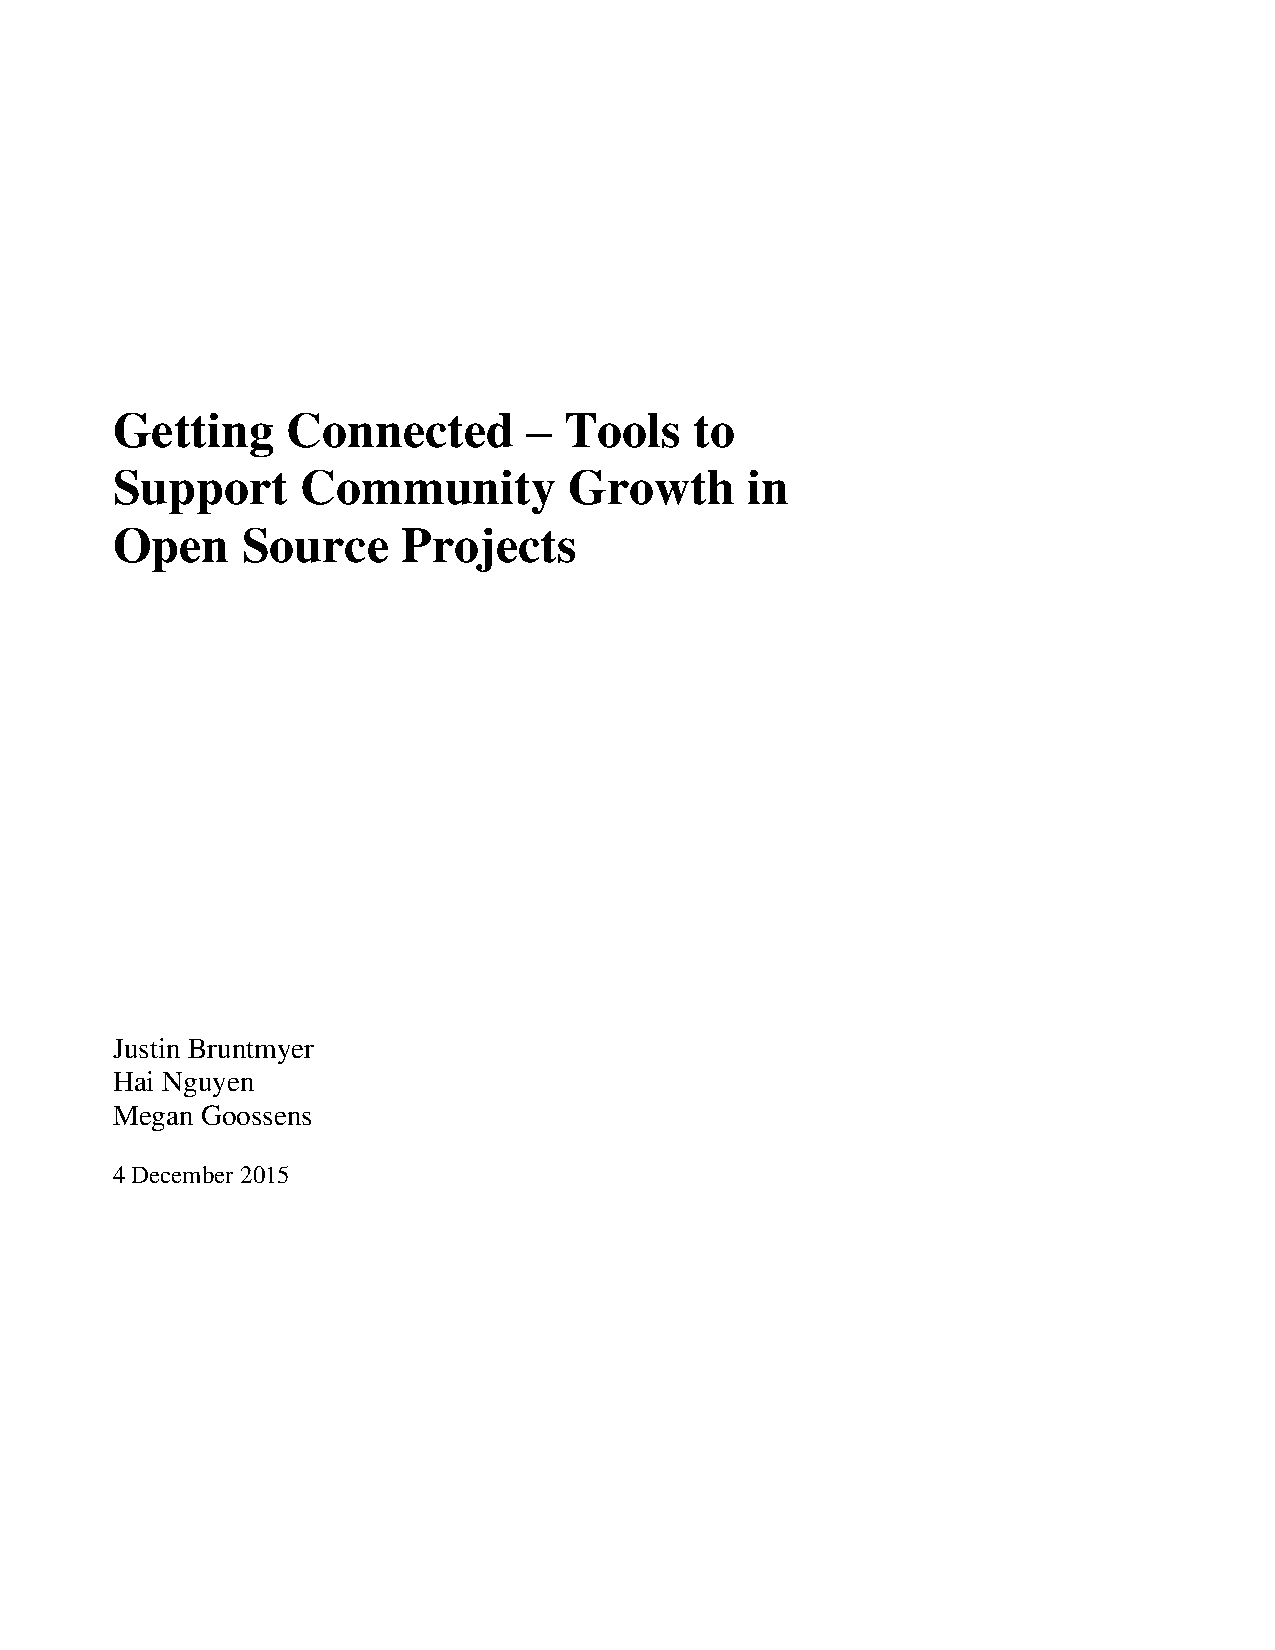
\includepdf[pages={1}, pagecommand={\section{DESIGN DOCUMENT}}]{Design_Document.pdf}
\includepdf[pages={2-}, pagecommand={}]{Design_Document.pdf}

\subsection{Discussion on Design Document}
Blah blah blah discussion will go here.

%Tech review is inserted here.

\includepdf[pages={1}, pagecommand={\section{TECHNOLOGY REVIEW}}]{technology_review.pdf}

\includepdf[pages={2-}, pagecommand={}]{technology_review.pdf}

\subsection{Discussion on Tech Review}
Blah blah blah discussion will go here.


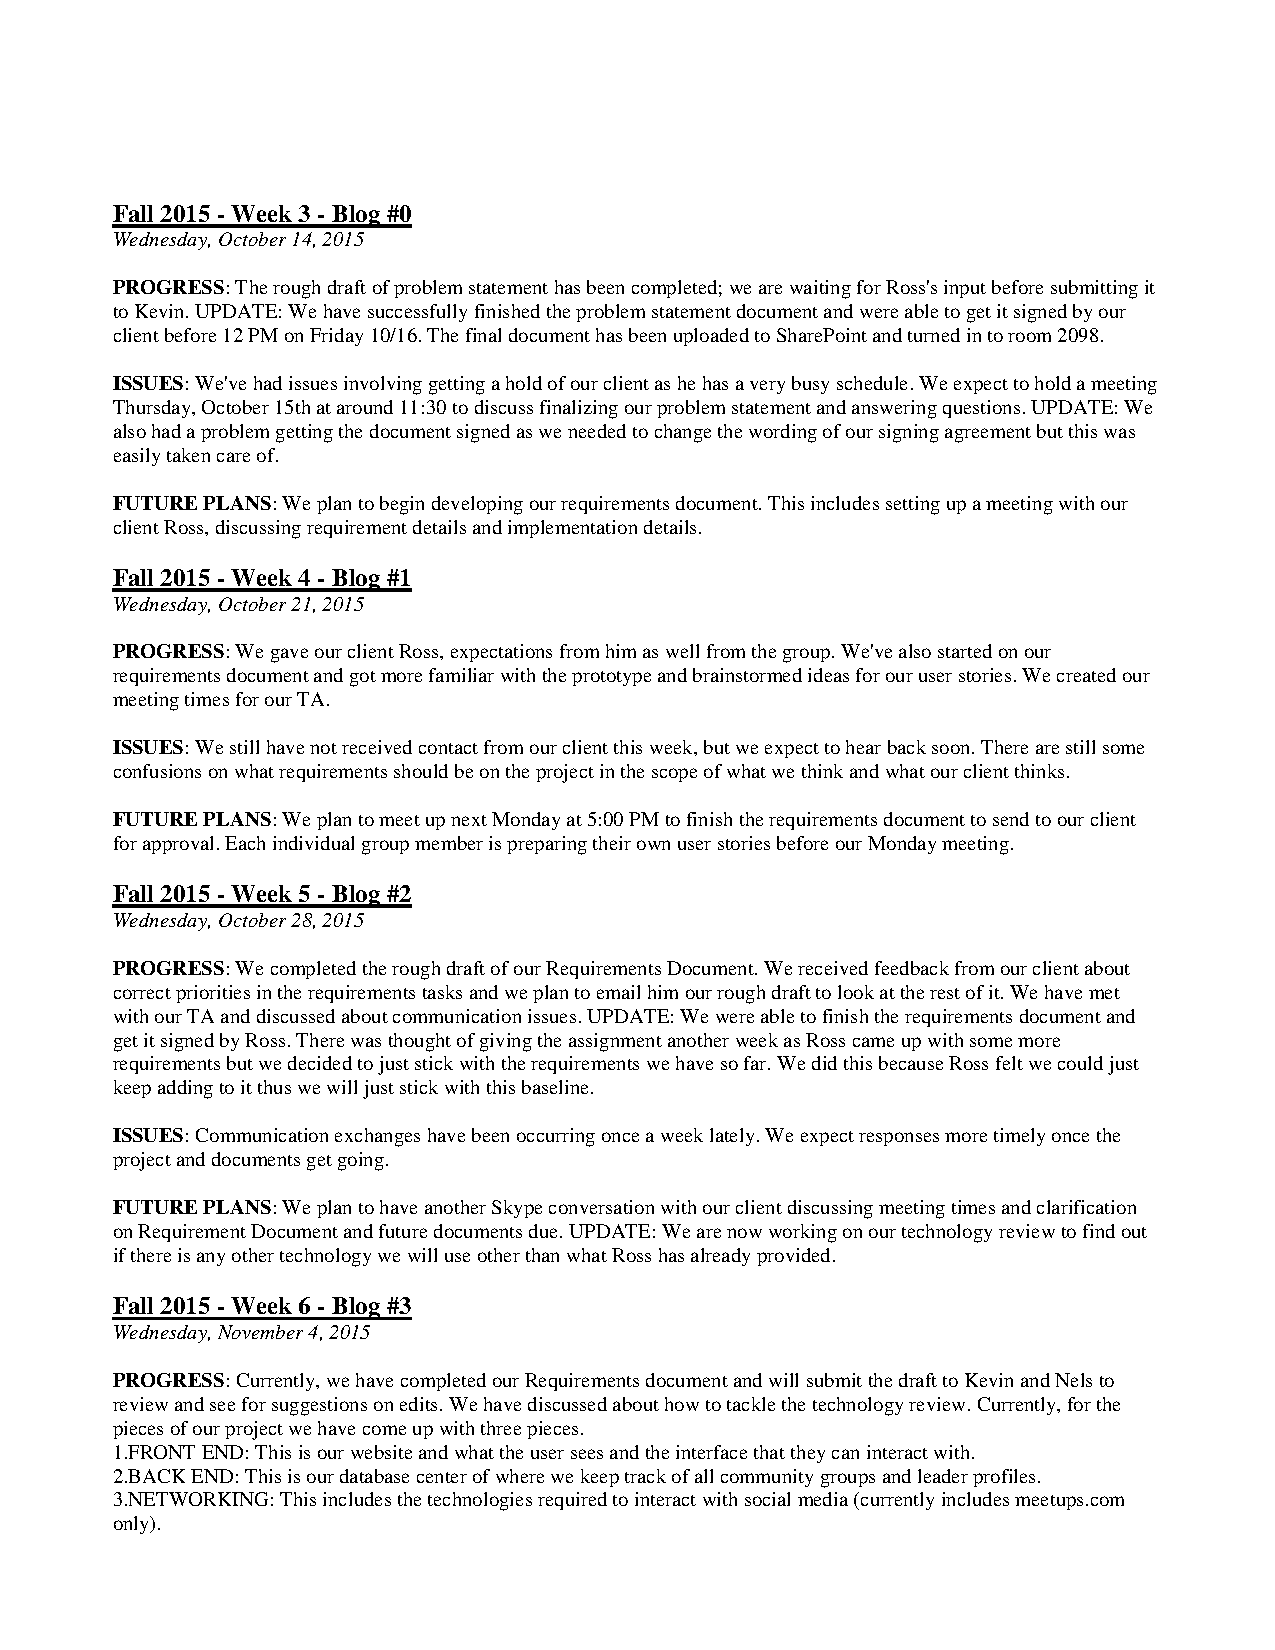
\includepdf[pages={1}, pagecommand={\section{BLOG POSTS}}]{Blog_Posts.pdf}
\includepdf[pages={2-}, pagecommand={}]{Blog_Posts.pdf}



\includepdf[pages={-}, pagecommand={}]{poster.pdf}

\section{PROJECT DOCUMENTATION}

\iffalse
\subsection{Fix the People page where the list of community leaders are shown}
\begin{enumerate}
  \item Completed Implementation: The “People” page currently takes all of the
    people in the database and lists them onto the page. Normally, if the
    prototype is hosted on a local machine and the database is relatively small,
    then the page loads fine in a minimal amount of time. The issue is nested in
    the actual hosted site by Apache where hundreds of thousands people are
    imported into the database daily and dramatically slowing down the loading
    time of the page.  With our current progression of the project, we have not
    made significant progress into improving the loading time of the page. We
    use our own local host to import a small amount of members at a time and
    that requirement is set to be worked on shortly for Beta implementation. The
    guideline for working towards accomplishing this requirement is to limit the
    amount of people loaded at a time onto the page. For Beta, we have
    rearranged where the table is generated for the people page in the function
    within views.py. This change specifically was introduced because a bug was
    found where when the table is generated, then if the amount of people were
    too many, then the table would crash and not build. With the rearrangement,
    now the table does not break through a large build and now tends to load
    faster. Unfortunately, the implementation of the fix for the People page is
    local. We have yet to test it on the host that Apache is using to run the
    prototype currently. We predict that the fix will work but it will need to
    be approved and patched into the live site for clarification.
\end{enumerate}
\fi

\iffalse
\subsection{Tweet at a person listed in the database}
\begin{enumerate}
  \item Completed Implementation: Each person who is imported into the application
    is generated their own profile page based off of their Meetups ID. Information from 
    Meetups about the person’s profile is also parsed in the community development tool. Those profiles
    include displaying the twitter handle of the person. This was done by changing
    the Meetup API request so that we could get the correct information and
    then store that information in our database. This can be seen in code snippet 1 located below 
    with the URL shown along with the 'if' statements to locate the twitter handle. This allows the user to get 
    in contact with the person in a profile. Above the
    twitter handle is a button that has the Twitter symbol which allows the user
    to click and send a tweet at the person via Hoot-suite. The hoot-suite app is
    given the twitter handle of the person the user wants to tweet at and the URL
    of the persons page on our application for reference. The user signs in to
    compose the tweet and sends it under their Twitter account. The code snippet 2 located below 
    shows the HTML encoding of the button used to create the Hootsuite connection and shows the 
    retrieval of the twitter handle form the database with 'person.service'. Not all users have a
    Twitter handle registered with Meetups thus the tweet button does not have any use. To handle this case
    the tweet at button only appears on profiles of imported people that have a registered Twitter handle.
\end{enumerate}
\fi  

\iffalse
\subsection{Add user accounts to application and track when a user has tweeted an event}
\begin{enumerate}
  \item Completed Implementation: The purpose of adding user accounts to the applications
    is to be able to track when users tweeting about events or people. With the completion
    of this requirement, the account creation is working along with being able to sign in 
    successfully with a confirmation of signing in by displaying a welcome message along with
    the user's username. There is also a login and logout button located in the
    top right section of the website on all pages allowing the user to login or
    logout at anytime. Everything is also backended with features of the website only existing
    if the user has an authorized account. This means that action functions within the application
    which include importing meetups, importing members, marking events as not
    applicable, and marking groups as not applicable to be behind being signed in.
    This means if you are not logged in with the authorized account, you can't perform these 
    actions. Note that the accounts created are allowed access to these features, but do not
    have access to the administrative page that deals with the Django database.

\end{enumerate}
\fi

\iffalse
\subsection{List tweets about events and/or people via the application}
\begin{enumerate}
  \item Completed Implementation: We were unable to track the precise tweets
    made from our application, but we have found an alternative that mostly
    works. As shown in the code snippet, the website makes a call to Twitter's
    search API, requesting all tweets that contain a certain hashtag as well as
    the hashtag \#Meetup. The hashtags are the same as the ones used to get
    events from meetup.com. Once it has the tweets, it uses the id from each one
    to make another call to Twitter's OEmbed API, which sends back HTML that is
    used in the page's template to present embedded tweets to users. This still
    pulls a few tweets that are unrelated, but bit of filtering would work.
    Unfortunately this would be difficult, and is outside the scope of our
    project.
\end{enumerate}
\fi

\iffalse
\subsection{List tweets about events and/or people not via the application}
\begin{enumerate}
  \item Completed Implementation: The website now has a tweet parser. As shown
    in the code snippet, it sends a call to Twitter's search API, requesting all
    tweets with a certain hashtag. The hashtags are the same as the ones used to
    get events from meetup.com. Once it has the tweets, it uses the id from each
    one to make another call to Twitter's OEmbed API, which sends back HTML that
    is used in the page's template to present embedded tweets to users.  The
    search results currently contain all instances of the hashtag requested,
    even when they are not relevant to any event, or even open source. The
    search needs refinement, however, this will be difficult, and is not within
    the scope of the project
\end{enumerate}
\fi

\iffalse
\subsection{Export a list of people with Information}
\begin{enumerate}
  \item Completed Implementation: When taking on this requirement we quickly realized that
    the Meetup API would not provide email address for its users which was
    understandable. We then looked at what other information would be useful to
    extract about the people that were loaded into the database. This lead us to
    export information such as name, twitter handle, bio, Meetup ID, URL, country,
    state, and city. The export can be executed by clicking on the 'Export Info'
    button located in the top left of the people page and creates a file in a XLSX
    format which can be directly opened or saved.
    
\end{enumerate}
\fi

\iffalse
\subsection{Improve hashtag searching of application to improve finding more relevant events}
\begin{enumerate}
  \item Completed Implementation: The solution to this issue was to change one word in
    the call to the meetup.com API. In the API there are many different
    restrictions you can use to request events. Two of them come into play here:
    "text" and "topic." The text query searches through the content of the
    events, while the topic query looks at the topics related to the group. The
    original query was looking at text, which resulted in a lot of unrelated
    events. The query was fixed to use "topic," which has reduced unwanted events
    significantly. A thourough examination of events imported resulted in no
    unrelated events pulled in.
\end{enumerate}
\fi

\newpage

\iffalse
\subsection{Improve the visuals of the tool's look as a whole}
\begin{enumerate}
  \item Completed Implementation: The application itself began as a fairly organized
  	piece. The navigation bar implementation really helps the user keep track navigating
  	between each page. When viewing the list of events, the events are listed in
  	chronological order starting with the most recent. There is a search bar
  	available for the user to type in for a certain event that they wish to view. There
  	are other sorting mechanisms to view those events in another sorting order.
  	Our focus in this requirement were to mainly to improve how data is displayed. This
  	specifically applies to to the event page and people profiles. Along with the addition
  	of the Host objects, the generated host profiles would have a visual update as well.
  	As displayed in Figure 9, the improvement of the profile page is shown with categories
  	specifically labelled and displayed in concrete areas of the page. If the certain variable
  	does not exist, then the user can clearly see where that detail would go on the page.
  	Topics are more clearly organized have are configured under a scrollable table as well.
  	Overall, this addition makes the people profile page much more organized and legible.
  	In addition to the updated people profile page, the event page is also upgraded in Figure
  	10. Similar to the profile upgrade, the event page now has categories that specifically
  	detail where objects belong. This is much more particularly important where the description
  	is displayed for the event. Previously, it was much more difficult for the user's eye to
  	view where the venue of event would be. Now in this update, that portion is clearly labelled
  	which allows the user to spend less time reading and to quickly see the information
  	that they want to. \\

\end{enumerate}
\fi

\iffalse
\subsection{Implement system of improved sorting of finding events by nearby location within radius of the user}
\begin{enumerate}
  \item Completed Information: This tool creates a list of all events parsed through 
    the application and displays a marker for each even onto the Google Map displayed
    to the right of the lists of events. A user can search for a specific event by looking
    through the list and then seeing where this is on the map. This feature also asks the 
    web browser of the user for the geo-location of the user in order to place a special
    marker on the map showing where the user is in reference to the rest of the markers. The
    user can decide weather or not to accept giving the their location to the application. The map
    is generated through Google Maps by using the Google Map API calls. This map was implemented 
    with a search bar allowing the user to search for a location and see what events are in 
    that location. With each search the map jumps to the searched location and is given a 200 mile radius
    circle to show what events are within 200 miles of the user. In order to get the markers of
    each event to show up on the map the latitude and longitude of each event needed to be stored and
    accessed by the map. This was done by a Meetups API call as shown in code snippet 3. Once the API call
    is made the json object is returned and parsed to obtain information on the event including name,
    longitude, and latitude. Once the information is stored it is accessed in the JavaScript for the 
    Google Map which can be seen in code snippet 4 below. This is done by looping though a list of 
    events and gather the name, longitude, and
    latitudes in order for the markers to display. When a user hovers over a marker on the map the name of
    the event is shown.  When there are no events imported a message stating 
    "No Events Available" is displayed.

\end{enumerate}
\fi


\iffalse
\subsection{Add feature to generate a profile for people and have it display a way to contact the person if a method is available}
\begin{enumerate}

  \item Completed Information: The main goal of the tool is to promote community
    development in the open source scene. What this feature tackles is a way to display
    important information about people that are already involved with projects to those
    who would like to get involved. This feature generates profiles for event hosts along
    with members of groups that have been imported by the user. These profiles consist of 
    the of selected person, Twitter handle, location, link to Meetups profile, last activity date, 
    group associated with, topics they are interested in, a biography, and a picture of themselves.
    In order to gather the information for these we had to make another API call to Meetups. First,
    we had to adjust the current API call for importing events to also gather the ID of the event hosts.
    Once this ID was obtained the next step is another API call gathering information on each event hosts
    while searching with the ID's gathered. Once this information was obtained the profiles for event
    hosts and imported group members could be displayed in their own sections of the application.
    With users having the options to see group members and event hosts there are more opportunities
    for these users to get involved.

\end{enumerate}
\fi


\section{How did you learn the new technology?}
Throughout the presentation of our tools to our client Ross Gardler we were happy to hear that he was really excited about the progress we have made thus far.
In his excitement in seeing how far we have come with the tools and the progress he has seen
Ross began asking for feature requests to be added to the tools we have developed thus far.
We decided to add this section to our report so that we could reference Ross's confidence in our team to make these requests possible if we have time.
These requests are for future ideas for the tools as our client also would like us to submit patches for the tools
that we have made thus far as he approves of the work we have done. We will be completing these patches and getting them to Ross.
The requirements that have had feature requests proposed are shown below.

\section{What did you learn from all of this? (Justin Bruntmyer)}

\subsection{What Technical Information Did I Learn}



\section{What did you learn from all of this? (Megan Goossens)}

\section{What did you learn from all of this? (Hai Nguyen)}


\section{PROBLEMS ENCOUNTERED}

Throughout this term we have encountered many problems that have impeded our
progress for this project. This was to be expected as with all projects. 
Events
occur that can halt progress and bring forth challenges that, as a group, we
needed to overcome. The problems that we have faced are listed below along with
the methods we used to get through the situation. We also ran into the occasioin coding block where we would have days where not much progress was obtained. However, we feel this did not impeded our progress as
it is just part of being a computer scientist.

\subsection{Problem 1}
Deciding which platform we were going to be developing on using Docker. This was
a major issue as we originally planed to work with the Windows operating system
however we could not get the application to run locally on a Windows platform.
We continually ran into errors with creating a local database along with having
the right Docker tools to support the application. We had available resources
such as a README file that gave insight on the problem but whatever we tried did
not seem to work. We eventually shifted gears and decided to try Docker and the
application on Linux, specifically Ubuntu 14.04. Thanks to the Linux knowledge
of Megan Goossens and plenty of online documentation we were able to get Docker
installed successfully along with running the application on a local host. From
this point we decided to continue developing in the Linux environment.

\subsection{Problem 2}
At the end of the Fall 2015 term we set up a weekly meeting with our client
throughout Winter 2016 to discuss implementation details for the week and
planned to utilize this time to make sure everyone is on the same page. Due to
some miss-communication we were unable to meet with our client for the first two
weeks. This halted our progress with because we had a lot of issues with getting
Docker to work with Windows and we were counting on a meeting with our client to
resolves those issues as soon as possible. We eventually got in contact with our
client and figured out what was happening as the first week our client was on an
unexpected trip to the UK and in the second week our client did not realize that
these meetings occurred every week throughout the term. These things happen and
once we all had a chance to get on the same page every weekly meeting is going
smoothly. This problem also happened at the beginning of the spring term. A new
weekly meeting time was set up with our client however our client believed that
our first meeting was in the middle of June. This was a problem as we tried to
set up a new meeting time but our client was very busy with travel and vacation
that we were not able to meet with him three weeks prior to expo. Email communication
was very difficult as well.

\subsection{Problem 3}
During week three of Winter 2016 we ran into the issue of meetings being
cancelled due to illness and injury. One of our team members experience an injury
that caused a full group meeting with a TA to occur which halted our progress in
having to get everyone caught up on the same page. This same week another group
member became sick and could not make it to two meetings for the week which
meant that two people could not make it so two meetings were cancelled out of the
weekly three meetings we have as a group. However, we were
able to work individually at home but it was still a noticeable disruption from
the normal work we produce in a week. It did not seem like it was going to
effect the group at first however when we began to get back on track it took
some adjustments to makes sure everyone was on the same page and try to make up
for the week we missed.

\subsection{Problem 4}
During the first week of the term we began developing based on the requirements
we had listed in our requirements document. The problem we ran into here was
that we had issues understanding what are requirements were trying to say thus
we went through the document and changed the language used for the requirements.
This did not change the requirement but it made it easier to understand if
someone is reading through it. This took a days worth of progress which was
frustrating due to the fact that we believed to have this done last term. We
currently are happy with the updated requirements document as it has been
approved by our client, professor, and TA. This halted our progress by being an
unnecessary step in the implementation process as it should have been completed
last term.

\end{document}
